% -*- TeX -*-

\documentclass{beamer}
\usepackage{amsmath}

\title{Crustal Deformation Modeling Tutorial}
\subtitle{}
\author{Brad Aagaard, Charles Williams, and Matthew Knepley}
\institute{
\includegraphics[scale=0.4]{../../logos/cig_blackfg}}
\date{June 20--24, 2011}


% ---------------------------------------------------- CUSTOMIZATION
\newcommand{\thispdfpagelabel}[1]{}
\newcommand{\important}[1]{{\bf\color{red}#1}}
\usetheme{CIG}

% --------------------------------------------------------- DOCUMENT
\begin{document}

% ------------------------------------------------------------ SLIDE
\maketitle

% ========================================================== SECTION
\section{Introduction}
\subsection{Agenda}

% ------------------------------------------------------------- LOGO
\logo{
\includegraphics[height=4.5ex]{../../logos/cig_blackfg}}

% ------------------------------------------------------------ SLIDE
\begin{frame}
  \frametitle{Workshop Instructors}
  \summary{}
  
  \begin{center}
    \begin{tabular}{ccc}
      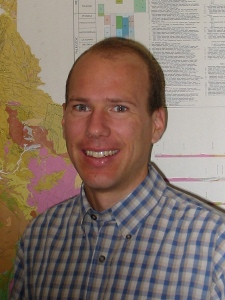
\includegraphics[width=1.2in]{figs/brad} & 
      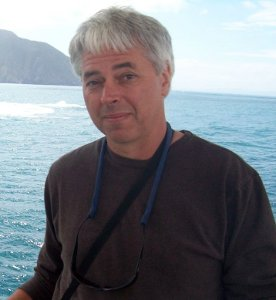
\includegraphics[width=1.2in]{figs/charles} &
      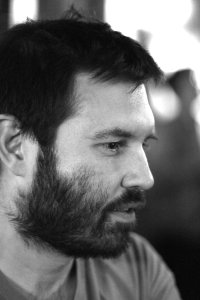
\includegraphics[width=1.2in]{figs/matt} \\
      Brad Aagaard & Charles Williams & Matthew Knepley \\
      USGS & GNS Science & Univ. of Chicago \\
      Menlo Park, CA & Lower Hutt, NZ & Chicago, IL
    \end{tabular}
  \end{center}

\end{frame}


% ------------------------------------------------------------ SLIDE
\begin{frame}
  \frametitle{Overview of Workshop}
  \summary{Draft agenda posted on geodynamics.org}
  
  \vfill
  \begin{center}
    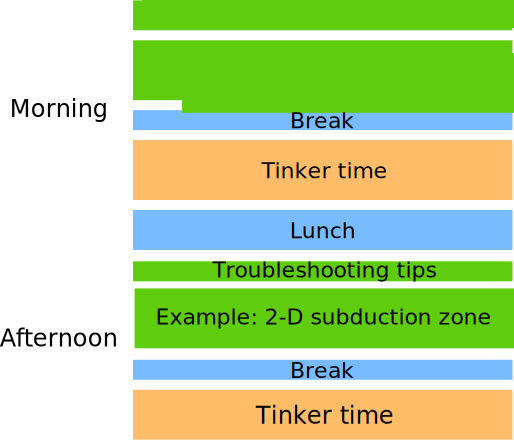
\includegraphics[width=4.5in]{figs/overview}
  \end{center}  

\end{frame}


% ========================================================== SECTION
\subsection{Adobe Connect}

% ------------------------------------------------------------ SLIDE
\begin{frame}
  \frametitle{Overview of Adobe Connect}
  \summary{}
 
  \begin{itemize}
  \item Audio input/output
    \begin{itemize}
    \item Participants microphones are muted by default
    \item Click on raised arm icon to ``Raise your hand''
    \item Your microphone will be enabled when hosts respond to your
      raised hand
    \end{itemize} 
  \item Q \& A Pod
    \begin{itemize}
    \item Submit questions using this tool.
    \item Adobe Connect tracks which ones have not been answered.
    \end{itemize}
  \item Chat Pod
    \begin{itemize}
    \item Useful for exchanging urls, text for commands, etc.
    \item Sessions will be recorded and archived for on-demand playback.
    \end{itemize}
  \end{itemize}

\end{frame}


% ------------------------------------------------------------ SLIDE
\begin{frame}
  \frametitle{CIG's First Online Tutorial}
  \summary{}
 
  \begin{center}
    {\Large\bf{\color{red} WARNING}}\\
    This is CIG's first attempt at an online tutorial. We have
    practiced using Adobe Connect but there may be bumps in the road!
  \end{center}

\end{frame}


% ========================================================== SECTION
\subsection{Getting Help}

% ------------------------------------------------------------ SLIDE
\begin{frame}
  \frametitle{Getting Help}
  \summary{}
 
  \begin{itemize}
  \item Read the PyLith manual
  \item Try to work through the problem on your own
  \item Submit questions to \important{\tt CDMhelp@geodynamics.org}
    \begin{itemize}
    \item Describe the problem
    \item Send complete error messages
    \item Include the platform you are using, the PyLith version, and
      whether it is a binary package or you built PyLith from source
    \item We will try to respond but may defer detailed responses to
      the next online session
   \end{itemize}
  \item Subscribe to \important{\tt cig-short@geodynamics.org}
    \begin{itemize}
    \item Answers to most questions will be cc'ed to this email list
    \item Short-term tectonics working group issues are posted here
    \end{itemize}
  \end{itemize}

\end{frame}

% ========================================================== SECTION
\subsection{CIG}

% ------------------------------------------------------------ SLIDE
\begin{frame}
  \frametitle{What is CIG?}
  \summary{Computational Infrastructure for Geodynamics
    ({\tt www.geodynamics.org})}
 
  \vfill

  Objective: Develop, support, and disseminate software for the
  geodynamics community.

  \vfill

  \begin{itemize}
  \item Coordinated effort to develop reusable, well-documented,
    open-source geodynamics software
  \item Strategic partnerships with the larger world of
    computational science and geoinformatics
  \item Specialized training and workshops for both geodynamics and
    larger Earth-science communities
  \end{itemize}

  \vfill
 
  Underlying principle: Earth scientists need help from computational
  scientists to develop state-of-the-art modeling codes

\end{frame}


% ------------------------------------------------------------ SLIDE
\begin{frame}
  \frametitle{CIG: Institution-Based Organization}
  \summary{Educational and not-for-profit organization}
 
  \begin{itemize}
  \item {\bf Open-organization}
    \begin{itemize}
    \item Any institution seeking to collaborate on the development of
      open-source geodynamics software
    \item No cost or size requirements
    \end{itemize}
  \item Current members
    \begin{itemize}
    \item 50 member institutions
    \item 10 foreign affiliates
    \end{itemize}
  \item NSF funding Jul 2010 -- Jun 2015
 \end{itemize}
\end{frame}


% ------------------------------------------------------------ SLIDE
\begin{frame}
  \frametitle{CIG Working Groups}
  \summary{Organized by sub-disciplines}
 
 \begin{itemize}
 \item Short-term tectonics
 \item Long-term tectonics
 \item Mantle convection
 \item Computational seismology
 \item Geodynamo
 \item Magma dynamics
 \end{itemize}

\end{frame}


% ------------------------------------------------------------ SLIDE
\begin{frame}
  \frametitle{Short-Term Tectonics Working Group}
  \summary{}
 
 \vfill
 
 \textbf{Objective}: Simulate crustal deformation across spatial
 scales from $1$ m to $10^3$ km and temporal scales ranging from
 $0.01$ s to $10^5$ years.

 \vfill
 \begin{itemize}
 \item Formed through efforts by Brad Hager and Mark Simons before CIG started
 \item Strong connection to SCEC Crustal Deformation Modeling focus group
 \item Building connections with SCEC Earthquake Source Physics focus group
 \end{itemize}
\vfill

\end{frame} 


% ------------------------------------------------------------ SLIDE
\begin{frame}
  \frametitle{CIG Organizational Structure}
  \summary{}
 
  \begin{itemize}
  \item Staff
    \begin{itemize}
    \item Responsible for software development
    \item Director handles day-to-day decisions
    \end{itemize}
  \item Science Steering Committee
    \begin{itemize}
    \item Voice of geophysics community
    \item Prioritizes the competing needs of all sub-disciplines
    \end{itemize}
  \item Executive Committee
    \begin{itemize}
    \item Primary decision-making body
    \item Approves SSC recommendations and contractual arrangements
    \end{itemize}
  \item Member institution representatives
    \begin{itemize}
    \item Vote on membership applications and bylaws
    \end{itemize}
  \item Community members
    \begin{itemize}
    \item Collaborate with staff to develop software
    \end{itemize}
  \end{itemize}

\end{frame}

% ------------------------------------------------------------ SLIDE
\begin{frame}
  \frametitle{CIG Activities}
  \summary{}

  \begin{itemize}
  \item Software development: primary activity
  \item Workshops
    \begin{itemize}
    \item Sponsors workshops organized by one or more working groups
    \item Holds workshops focusing on scientific computing and geodynamics
    \end{itemize}
  \item Training in use of CIG software
    \begin{itemize}
    \item Tutorials at workshops
    \item Specialized training sessions (like this one)
    \end{itemize}
  \item Web site: {\tt geodynamics.org}
    \begin{itemize}
    \item Distribution of software and documentation
    \item Mailing lists for each working group
    \item Wiki-like web pages for community involvement
    \end{itemize}
  \end{itemize}
 
\end{frame}


% ------------------------------------------------------------ SLIDE
\begin{frame}
  \frametitle{CIG Software}
  \summary{}

  \vfill
  \begin{center}
    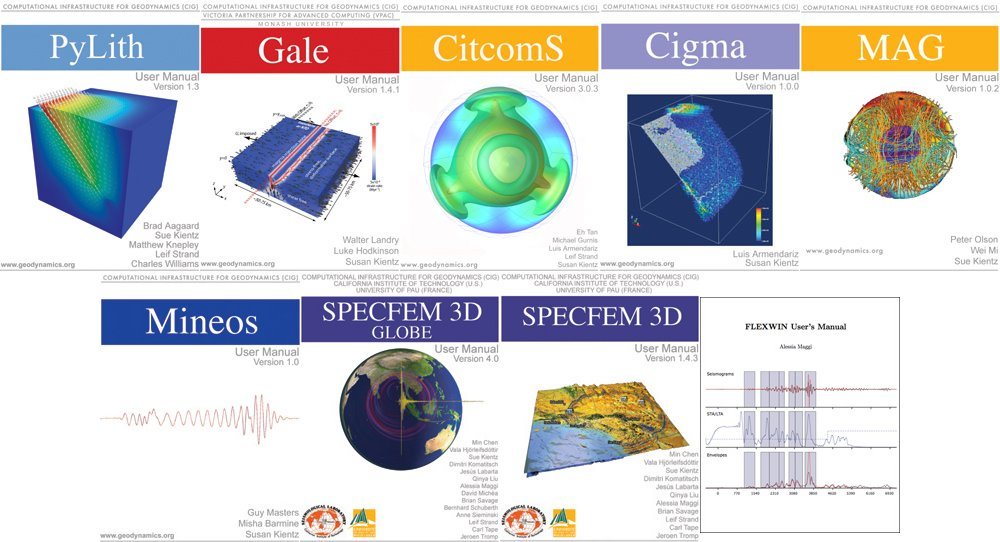
\includegraphics[width=4.5in]{figs/covers}
  \end{center}
  \vfill

\end{frame}

% ------------------------------------------------------------ SLIDE
\begin{frame}
  \frametitle{CIG Software for Crustal Deformation}
  \summary{}

  \begin{itemize}
  \item PyLith
    \begin{itemize}
    \item Solves 2-D and 3-D problems associated with earthquake
      faulting and quasi-static and dynamic viscoelastic deformation
    \item Short-term tectonics where geometry does not change
      significantly
    \end{itemize}
  \item Gale
    \begin{itemize}
    \item Solves problems in orogenesis, rifting, and subduction,
      including free surfaces with coupling to surface erosion models
    \item Long-term tectonics where geometry changes significantly
    \end{itemize}
  \end{itemize}
 
\end{frame}

 
% ======================================================================
\end{document}


% End of file
